\section{Motivation}


\begin{figure}[t]
	\centerline{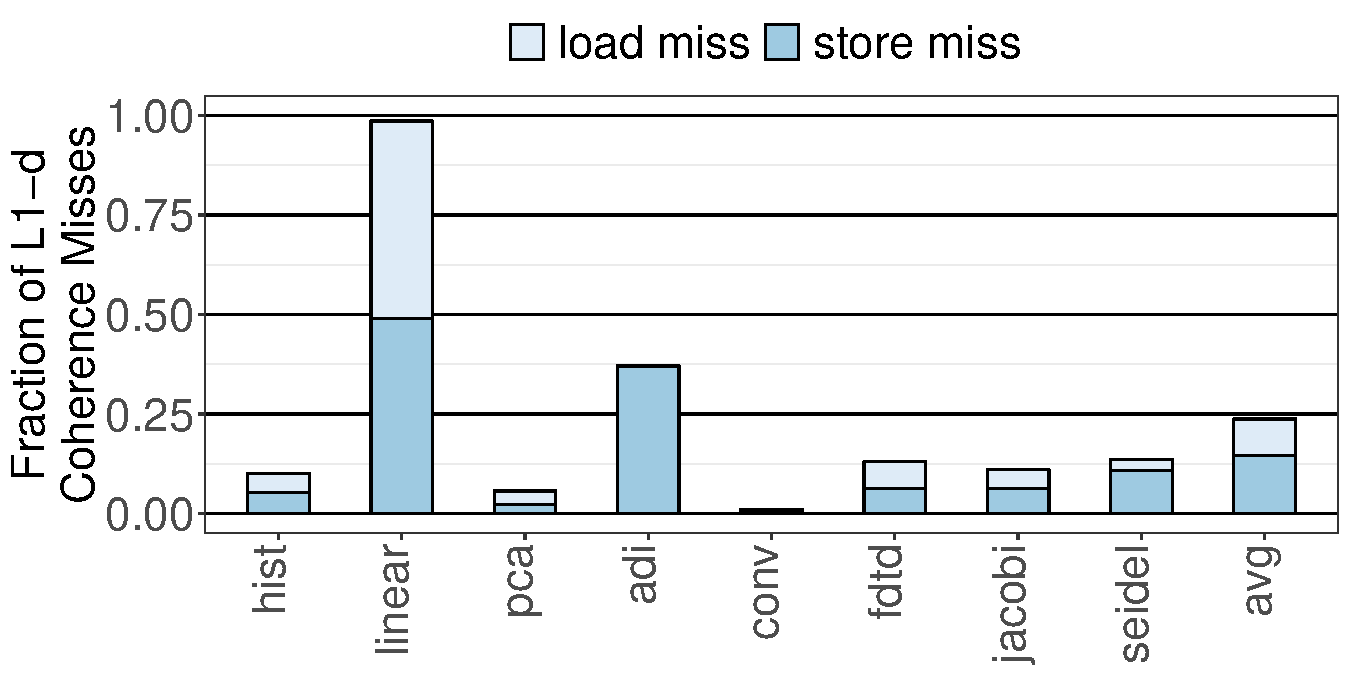
\includegraphics[scale=0.4]{graphs/coherence_misses_L1.pdf}}
	\caption{L1-d coherence misses normalized to total amount of cache misses.}
\label{fig:coherence_misses}
\end{figure}

\begin{table}[t]
\caption{Percent difference in store values of benchmarks.}
\begin{tabular}{|llll|}
\hline
\textbf{Benchmark} & \textbf{Suite} & \textbf{Input Size} & \textbf{\% Diff.	}\\ \hline

histogram & Phoenix 2.0 & 400MB (medium) & 0.011 \\

linear\_regression & Phoenix 2.0 & 100MB (medium) & 0.005 \\

pca & Phoenix 2.0 & 4MB (medium) & 18.967 \\

adi & Polybench &  TODO (small) & TODO \\

conv-3d & Polybench & TODO (small) & TODO\\

fdtd-apml & Polybench & TODO (small) &  TODO\\

jacobi-2d & Polybench & TODO (small) & TODO\\

seidel-2d & Polybench & TODO (small) & TODO\\ \hline

Average &  &          & avg\_val\\ \hline
\end{tabular}
\label{tab:benchmarks}
\end{table}

% {\color{red} Include a table with benchmarks and the average total percent difference in the store values}


% {\color{red} Include a figure with the normailized amount of coherence misses}


% \begin{itemize}
% 	\item Some computing applications have large fraction of cache misses due to coherence due to false/true sharing
% 	\item Define we characterize coherence misses. Tag match but in the wrong coherence state.
% 	\item Cache misses slow down performance, increase network traffic and increase energy consuption.
% 	\item These application also show low percent difference between consecutive computation data store values.
% 	\item These application might be used in error-tolerant applications. I.e multimedia, image processing, machine learning.
% 	\item We relax the coherence protocol to leverage this. 
% 	\item Since consective store values show high similarity we can avoid coherence requests to reduce latency and energy consumption. 
% \end{itemize}

Many parallel applications experience a significant amount of contention on shared data structures. In a coherence protocol, contention of shared data occurs when multiple cores request exlusive access to the same cache line. In an invalidation based protocol, if one core requests exclusive access, then all other copies of that data in private caches of other cores' must be invalidated. Subsquest accesses to the invalidated data would results in cache misses which not only incurs latency, but also greater energy consumption due to increased coherence traffic and cache-to-cache data transfers.

We sample several application kernels from the Phoenix 2.0 \cite{phoenix} and Polybench Suites \cite{polybench} (see Table \ref{tab:benchmarks}). These kernels are selected for their ameniblity to approximation and being able to complete on our simulator. Figure \ref{fig:coherence_misses} shows a breakdown of the fraction of coherence cache misses. We define coherence cache misses as misses when the tag is present in the cache, but in the wrong coherence state (i.e., Stores on read-only/invalid or Loads on invalid). On average for our sampled applications, a sizeable 23.7\% of the L1-d misses are due to lines being in the wrong coherence state -- with 61.7\% of those misses coming from store instructions. Stores contribute to a larger portion of coherence misses due to the stricter conditions for a hit; the cache line must be held exclusively by the current node which means in a standard MOESI protocol, stores would miss in $\frac{3}{5}$ stable states. Upon a store miss, the protocol would request for exclusive access (GetX) and Invalidate (Inv) all other shared copies of the cache line. In contrast, a load miss would only send out a shared request (GetS) without invalidating other copies. We also look at the percent difference of store values of computation data compared to its last stored value shown in Table. \ref{tab:benchmarks}. On average the percent difference of the store values is avg\_val\% which corresponds to high approximate value locality \cite{lva}. Stores not only make up a larger fraction of coherence misses but also generate more coherence traffic, hence we target stores to exploit the approximate value locality within error-tolerant applications.

